\documentclass[tikz,border=2pt]{standalone}
\renewcommand{\familydefault}{\sfdefault}
\usetikzlibrary{arrows.meta,calc,positioning}
\tikzset{every picture/.style={line width=1pt, >=Stealth},
         hl/.style={fill=black, fill opacity=0.12, text opacity=1}}
\begin{document}
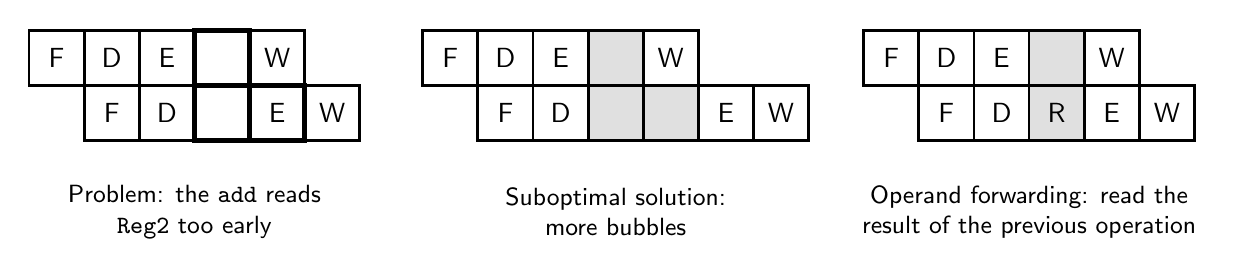
\begin{tikzpicture}[x=0.7cm, y=0.7cm, cell/.style={draw, minimum size=0.7cm},
    stall/.style={hl}, clash/.style={line width=1.8pt}]
  % \pipe{row}{first cycle}{stage/style, ...}: one instruction, one cell per clock cycle
  \newcommand{\pipe}[3]{\foreach \v/\s [count=\i from 0] in {#3} \node[cell, \s] at (#2 + \i, -#1) {\v};}
  % The second instruction needs a register the first has not written back yet (bold).
  \pipe{0}{0}{F/, D/, E/, /clash, W/}
  \pipe{1}{1}{F/, D/, /clash, E/clash, W/}
  \node[font=\small, align=center] at (2.5, -2.8) {Problem: the \texttt{add} reads \\ \texttt{Reg2} too early};
  \begin{scope}[xshift=5cm]
    \pipe{0}{0}{F/, D/, E/, /stall, W/}
    \pipe{1}{1}{F/, D/, /stall, /stall, E/, W/}
    \node[font=\small, align=center] at (3, -2.8) {Suboptimal solution: \\ more bubbles};
  \end{scope}
  \begin{scope}[xshift=10.6cm]
    \pipe{0}{0}{F/, D/, E/, /stall, W/}
    \pipe{1}{1}{F/, D/, R/stall, E/, W/}
    \node[font=\small, align=center] at (2.5, -2.8) {Operand forwarding: read the \\ result of the previous operation};
  \end{scope}
\end{tikzpicture}
\end{document}
